\documentclass[11pt,a4paper]{article}
\usepackage[utf8]{inputenc}
\usepackage[T1]{fontenc}
\usepackage[english]{babel}
\usepackage[margin=2.1cm]{geometry}
\usepackage{booktabs,array,tabularx}
\usepackage{xcolor}
\usepackage{graphicx}
\usepackage{pgfplots}
\pgfplotsset{compat=1.17}
\PassOptionsToPackage{hyphens}{url}
\usepackage[hidelinks]{hyperref}
\usepackage{enumitem}
\setlist{nosep,leftmargin=1.4em}
\emergencystretch=3em

\definecolor{impl}{HTML}{3B6EA8}
\definecolor{rev}{HTML}{8FB3DA}
\definecolor{waste}{HTML}{C0504D}

\title{Sweatshop on P-Chess: lane \texttt{core}\\\large The rules engine and the first playable board (CORE-002 to CORE-005, UI-001), plus the Lc0 bridge (BOT-002); night lineup, Opus 5.5 throughout}
\author{Foreman, session \texttt{sweatshop/core/2026-10-24-0159}}
\date{24 October 2026}

\begin{document}
\maketitle

\section*{Summary}

Lane \texttt{core} ran in the clone \path{.artifacts-build/lanes/core}, started from
\texttt{main} at \texttt{ed150e5} (CORE-001 merged by the \texttt{skeleton} lane), alongside
the \texttt{bot} and \texttt{skeleton}/\texttt{side} lanes. Lineup \texttt{-Lineup night}
(binding \texttt{1860cc4}): stage 2 \texttt{opus-5.5 high}, hard \texttt{opus-5.5 xhigh},
stage 3 \texttt{opus-5.5 xhigh}. Two launches: 01:59 (pid 12844, ended 03:30) and 03:31 (pid
12384, ended 03:59 with ``Nothing runnable'').

\begin{itemize}
  \item \textbf{Produced:} \textbf{5 tickets approved} on the session PR
        \href{https://github.com/Laginho/P-Chess/pull/3}{\#3}: CORE-002, CORE-003, CORE-004,
        CORE-005, UI-001, all \texttt{Review: agent}, \texttt{Verdict: Approve}. BOT-002 is
        merged on the session with \texttt{Verdict: Needs your call} and parked
        \texttt{blocked}.
  \item \textbf{Cost:} \textbf{\$35.99} at API list price over 16 stages, all priced:
        \texttt{opus-5.5 high} \$7.30 (stage 2), \texttt{opus-5.5 xhigh} \$28.69 (\$13.04 hard
        stage 2, \$15.65 review). Claude models only: Codex quota \texttt{--}. One Codex
        thread ran outside the stages (the attribution judge, \texttt{gpt-6-astra medium},
        24k tokens).
  \item \textbf{What went wrong:} the PR cannot be merged under the night's agent-only rule,
        because BOT-002 needs a real Lc0 that this machine does not have (BOT-001, the fetch
        script, is a \texttt{Review: human} ticket in the \texttt{mvp} lane). The
        \texttt{side} lane's CORE-005 and UI-001 are therefore not on \texttt{main}.
  \item \textbf{Provisional verdict:} the night lineup worked: one reopen in five tickets, a
        real defect, fixed in one cycle. Every lost attempt came from the environment
        (permissions, missing engine) or the driver (receipt parsing), not from the model.
\end{itemize}

\section*{What was done}

\textbf{CORE-002}: the game now has a position it can read and write as FEN, and the
position key that repetition and the opening book match on. Main file
\path{core/board.gd}. A 19+ digit move counter is clamped with an engine error instead of
rejected; deferred by the proxy.

\textbf{CORE-003}: legal move generation, verified by perft against every Chess Programming
Wiki count (start position to depth 4, Kiwipete and positions 3--6). Moves are UCI strings,
the form the Lc0 bridge speaks. Beyond the criteria, the en-passant square is written only
when a legal capture exists (as Lichess does), so repetition counts match. Main file
\path{core/board.gd}.

\textbf{CORE-004}: a game knows when it is over: checkmate, stalemate, the 50-move rule,
fivefold, threefold claim (with \texttt{auto\_claim}), insufficient material following
scalachess, flag and resignation, each with a PGN result and reason. Main file
\path{core/game.gd}. Attempt 1 wrote the whole thing but could not record its gate receipt
(permissions); attempt 2 reused the saved commits.

\textbf{CORE-005}: SAN in and out: \texttt{san()} prints moves with correct disambiguation,
check and mate marks; \texttt{parse\_san()} reads them back. \emph{Reopen:} a pawn move
written without its file (\texttt{d5} after 1.e4 d5) was read as the capture
\texttt{exd5} instead of an error; the cause was \texttt{parse\_san} not tying a fileless pawn
move to the destination file, in \path{core/board.gd}. Fixed in one cycle (3 lines).

\textbf{UI-001}: the first playable screen: two people play on a draggable board with a SAN
move list, flip, 1280$\times$800 window with an 800$\times$600 minimum. Main files
\path{ui/board_view.gd} and the main scene. The cburnett piece SVGs were reproduced from
their path data (no network) and must be replaced with the Commons originals before
integration; no human has played a game on it yet.

\textbf{BOT-002}: \path{engine/uci.gd} starts Lc0 once, reads it on worker threads and returns
Maia's move probabilities. Built on a fixture rebuilt from Lc0 v0.32.1's documented format,
not recorded; the live process code has never run. Needs a human with Lc0 installed.

\section*{Timeline}

\begin{tabularx}{\linewidth}{@{}lX@{}}
\toprule
01:35 & Clone made; waiting for CORE-001 on \texttt{main}. \\
01:59 & CORE-001 merged (PR \#1); driver launched, pid 12844. \\
02:02--02:53 & CORE-002, CORE-003, CORE-004 merged on the session; CORE-004 lost attempt 1 to a permission denial on \texttt{gate-evidence.ps1}. \\
03:05 & CORE-005 reopened (pawn SAN without file). \\
03:08 & CORE-005 fix parked by the driver: two \texttt{Gate evidence:} lines, the driver read the stale one. \\
03:10--03:30 & BOT-002: attempt 1 asked about Lc0; proxy chose a rebuilt fixture; review merged it as \emph{Needs your call}; driver parked it (review edited BOT-004's ticket after the gate). Run ends, PR \#3 opened. \\
03:31 & Foreman renames the stale receipt, restores CORE-005 to \texttt{to-review}; relaunch, pid 12384. Parent session: leave PR \#3 for Bruno, no revert. \\
03:38--03:59 & CORE-005 and UI-001 merged on the session. Nothing runnable. \\
\bottomrule
\end{tabularx}

\section*{Per stage}

{\small
\begin{tabularx}{\linewidth}{@{}llllrrrrrX@{}}
\toprule
When & Ticket & Stage & Model & Min & In & Cache & Out & Cost & Outcome \\
\midrule
02:02 & CORE-002 & impl & high & 3 & 2.0M & 97\% & 17k & 1.19 & to-review \\
02:11 & CORE-002 & review & xhigh & 8 & 3.4M & 94\% & 52k & 2.27 & merged \\
02:20 & CORE-003 & impl & xhigh & 9 & 3.5M & 97\% & 49k & 2.50 & to-review \\
02:31 & CORE-003 & review & xhigh & 11 & 3.2M & 92\% & 69k & 2.54 & merged \\
02:38 & CORE-004 & impl & xhigh & 8 & 3.6M & 97\% & 44k & 2.38 & failed (permissions) \\
02:46 & CORE-004 & impl & xhigh & 7 & 5.7M & 97\% & 38k & 2.98 & to-review \\
02:53 & CORE-004 & review & xhigh & 8 & 3.8M & 94\% & 53k & 2.46 & merged \\
02:58 & CORE-005 & impl & high & 5 & 2.7M & 97\% & 24k & 1.62 & to-review \\
03:05 & CORE-005 & review & xhigh & 7 & 2.4M & 94\% & 48k & 1.73 & reopened \\
03:08 & CORE-005 & impl & high & 2 & 1.7M & 97\% & 9k & 0.86 & parked (driver) \\
03:10 & BOT-002 & impl & xhigh & 2 & 1.4M & 96\% & 12k & 0.99 & failed (asked) \\
03:24 & BOT-002 & impl & xhigh & 14 & 6.0M & 97\% & 81k & 4.18 & to-review \\
03:30 & BOT-002 & review & xhigh & 6 & 3.6M & 94\% & 52k & 2.30 & parked (driver) \\
03:38 & CORE-005 & review & xhigh & 7 & 3.4M & 96\% & 39k & 1.84 & merged \\
03:50 & UI-001 & impl & high & 12 & 5.3M & 97\% & 68k & 3.63 & to-review \\
03:59 & UI-001 & review & xhigh & 9 & 4.8M & 96\% & 53k & 2.52 & merged \\
\midrule
 & & & & 118 & 56.5M & & 708k & 35.99 & \\
\bottomrule
\end{tabularx}
}

All models are \texttt{opus-5.5}. Input is almost entirely cache reads (92--97\%), so the
input volume is cheap; cost follows output and effort.

\begin{center}
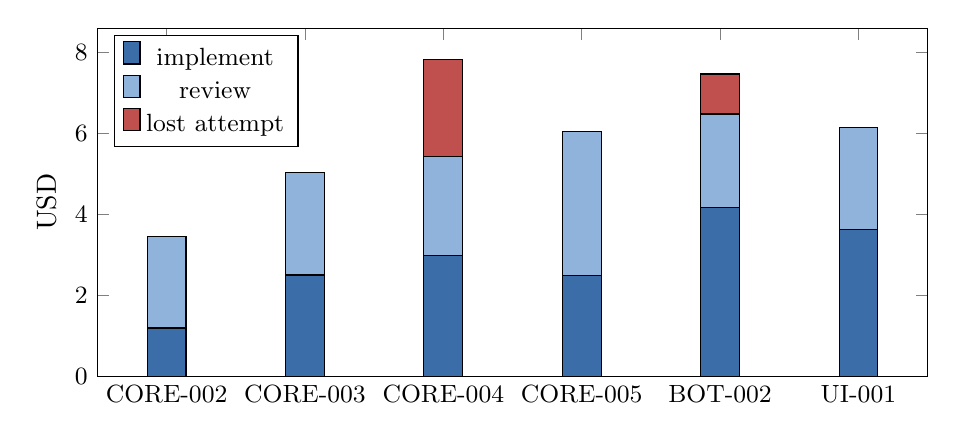
\begin{tikzpicture}
\begin{axis}[ybar stacked, bar width=14pt, width=\linewidth, height=6cm,
  symbolic x coords={CORE-002,CORE-003,CORE-004,CORE-005,BOT-002,UI-001},
  xtick=data, ylabel={USD}, ymin=0, legend style={at={(0.02,0.98)},anchor=north west,font=\small},
  tick label style={font=\small}]
\addplot[fill=impl] coordinates {(CORE-002,1.19) (CORE-003,2.50) (CORE-004,2.98) (CORE-005,2.48) (BOT-002,4.18) (UI-001,3.63)};
\addplot[fill=rev] coordinates {(CORE-002,2.27) (CORE-003,2.54) (CORE-004,2.46) (CORE-005,3.57) (BOT-002,2.30) (UI-001,2.52)};
\addplot[fill=waste] coordinates {(CORE-002,0) (CORE-003,0) (CORE-004,2.38) (CORE-005,0) (BOT-002,0.99) (UI-001,0)};
\legend{implement, review, lost attempt}
\end{axis}
\end{tikzpicture}
\end{center}

Lost attempts: \$3.38 (9\% of the run): CORE-004 attempt 1 (permission denial; its commits
were reused) and BOT-002 attempt 1 (asked about Lc0). CORE-005's reopen cycle cost \$4.43
(review \$1.73, fix \$0.86, re-review \$1.84) and is counted as work, not waste.

\section*{Comparison with previous runs}

\texttt{run-log.md} holds two earlier lanes from tonight: \texttt{skeleton} (CORE-001: two
\texttt{haiku-5.5 high} attempts that never invoked ticket-flow, then \texttt{opus-5.5 high};
\$5.61) and \texttt{bot} (BOT-003, \texttt{opus-5.5 xhigh}, \$4.87, no reopen). Per approved
ticket, \texttt{core} cost \$7.20 (BOT-002's stages included), against \$5.61 and \$4.87; its tickets
were larger (move generation, rules, a UI).

\section*{Observations per model}

\begin{itemize}
  \item \textbf{opus-5.5 high (stage 2)}: 4 runs, 3 to review in 3--12 minutes. One real
        defect missed (CORE-005, S2 explicit). Fast and cheap: \$1.19--\$3.63 per
        implementation.
  \item \textbf{opus-5.5 xhigh (hard stage 2)}: CORE-003, CORE-004, BOT-002. Perft correct on
        the first green run. Both of its failed attempts were environmental.
  \item \textbf{opus-5.5 xhigh (review)}: 6 reviews. It found the CORE-005 defect with a
        Godot probe, and on CORE-005's re-review it rebased onto the moved session and reran
        the gate instead of trusting a stale receipt. It never reopened for noise. Its two
        weak points: on BOT-002 it edited BOT-004's ticket after the gate, which parked a
        valid merge; and on UI-001 it added a comment to CI-002's ticket in
        \path{.scratch/mvp}, a folder no lane was to touch tonight.
\end{itemize}

\section*{Driver and runtime issues}

\begin{enumerate}
  \item \textbf{Permission shape of the gate-evidence helper.} Only a single Bash command
        that starts with \texttt{powershell -NoProfile -File} is allowed; \texttt{\&},
        \texttt{powershell.exe}, a leading \texttt{cd} or a variable are denied. Cost
        CORE-004 one attempt (\$2.38). Same issue in the \texttt{bot} lane (BOT-003).
  \item \textbf{First \texttt{Gate evidence:} line wins.} \texttt{Field()} in
        \path{driver.ps1} takes the first match. A reopened ticket keeps attempt 1's receipt
        above the new one, so a valid fix is parked as ``code changed after gate''. Fixed by
        hand (rename to \texttt{Gate evidence (superseded, attempt 1):}).
  \item \textbf{Any file changed after the gate parks the handoff,} including another ticket's
        \texttt{.md}: BOT-002's review routed comments into BOT-004's ticket and was parked
        after merging.
  \item \textbf{No Lc0 in lane clones.} \path{engine/} is gitignored and absent everywhere;
        BOT-002's implicit dependency on BOT-001 is not in its \texttt{Blocked by}.
\end{enumerate}

\section*{Recommendations}

\begin{enumerate}
  \item State the allowed \texttt{gate-evidence.ps1} invocation in \texttt{ticket-flow}
        (one line), or allow \texttt{\&} calls of that script in the driver's
        \texttt{--allowedTools}.
  \item Make the driver read the \emph{last} \texttt{Gate evidence:} line, or have stage 2
        rename the previous receipt when it writes a new one.
  \item Let a review's edits to \emph{other tickets'} \texttt{.md} files pass the
        ``code changed after gate'' check: they are not code.
  \item Add BOT-001 to BOT-002's \texttt{Blocked by}, or run BOT-001 before any lane that
        needs Lc0.
  \item Keep the night lineup (Opus high/xhigh) for spine tickets; the haiku-5.5 stage 2 is
        not usable with ticket-flow (CORE-001). Evidence: rows
        \texttt{opus-5.5 high \textrightarrow{} opus-5.5 xhigh} (4 reviews, an anecdote) and
        \texttt{haiku-5.5 high} (15 failed of 26).
\end{enumerate}

\section*{Human debt and proxy decisions}

No \texttt{Débito humano:} lines this run. \texttt{Proxy decided} lines, all by Opus:

\begin{itemize}
  \item \textbf{CORE-002}: ``defer the int64-overflow counter path in Board.from\_fen with no
        follow-up ticket''; nothing crashes and no planned feature sends outside FENs.
  \item \textbf{CORE-003}: ``defer both en-passant findings in Board.from\_fen with no
        follow-up ticket''; only an outside FEN reaches them.
  \item \textbf{CORE-004}: retry \texttt{gate-evidence.ps1} once in the allowlisted
        \texttt{powershell -NoProfile -File} form, no hand-made receipt. And: ``defer the
        null-board crash in Game.new(fen)'' with the other outside-FEN deferrals.
  \item \textbf{BOT-002}: ``option A'': build on a fixture rebuilt from the v0.32.1 format,
        labelled, with Acceptance pending until it is re-recorded from real Lc0.
  \item \textbf{UI-001}: ``reproduce the 12 cburnett SVGs from the known path data'',
        labelled in \path{docs/THIRD_PARTY.md}, Acceptance pending integration.
\end{itemize}

The three outside-FEN deferrals share one trigger: the first ticket that lets a user paste a
FEN must fix all three. I checked every ticket in \path{.scratch/}: none does today.

\section*{Reopen attribution}

\begin{tabularx}{\linewidth}{@{}llXlX@{}}
\toprule
Ticket & Round & Finding & Label & Why \\
\midrule
CORE-005 & 1 & \texttt{parse\_san} read a fileless pawn SAN as a capture & S2-explícito/código & Criterion 3: illegal or ambiguous SAN returns an error. Judged by \texttt{gpt-6-astra medium}, since the reviewer is Opus. Review miss: no; churn: no. \\
\bottomrule
\end{tabularx}

\medskip
Totals: S2-explícito/código 1. No fixes in review that added proof or behaviour (UI-001's
review commit \texttt{2ddc70e} changed comments and docs only). No session-review,
release-audit or post-release findings yet.

\section*{Scoreboard}

\texttt{scoreboard.ps1} over P-Chess (read from the lane clone, whose log is identical to the
main checkout's after the copy-back and which also holds this run's attribution file),
ClassyCall, EasyMath, PhysiSyst, SIGAA-ME, SynchroNice and slip. Rows that moved tonight,
all new: \texttt{opus-5.5 high} (7 runs), \texttt{opus-5.5 xhigh} (14 runs), and the pairs
below. Every Opus 5.5 pair is under 10 reviews: anecdotes.

{\small
\begin{tabular}{@{}llrrrrr@{}}
\toprule
Implementer & Reviewer & Reviews & Reopened & Rate & S2 & S2 rate \\
\midrule
opus-5.5 high & opus-5.5 xhigh & 4 & 1 & 25\% & 1 & 25\% \\
opus-5.5 xhigh & opus-5.5 xhigh & 3 & 0 & 0\% & 0 & 0\% \\
? & opus-5.5 xhigh & 2 & 0 & 0\% & 0 & 0\% \\
\midrule
gpt-6.1-sol high & gpt-6.1-sol xhigh & 87 & 12 & 14\% & 11 & 13\% \\
gpt-6.1-sol high & gpt-6.1-sol max & 94 & 21 & 22\% & 20 & 21\% \\
\bottomrule
\end{tabular}
}

\medskip
Implementers: \texttt{opus-5.5 high} 7 runs, 5 to review, 2 failed, median 5 min, \$11.85;
\texttt{opus-5.5 xhigh} 14 runs, 10 to review, 4 failed, median 14 min, \$81.43;
\texttt{haiku-5.5 high} 26 runs, 6 to review, 15 failed, 5 asked. Interventions recorded
across repos: 21 human rescues, 45 automatic recoveries, 14 Opus proxy decisions (6 from
this run), 1 routine approval. The full printout is in the run's scratch output; the rows
above are the ones this run touched plus the binding's default pair for comparison.

\section*{Pending for the human}

\begin{enumerate}
  \item PR \#3 is not merged. Either integrate BOT-002 after re-recording its Lc0 fixture and
        running the gate with \path{engine/} present, or revert its merge on the session
        (\texttt{git revert -m 1 8a8cf74}) and merge the rest; the \texttt{side} lane is
        waiting for CORE-005 and UI-001.
  \item UI-001: fetch the Commons piece SVGs (command in the ticket), look at the board, and
        play one game by hand.
  \item BOT-002 \texttt{PolicyTemperature}: one value for the move picker, premove check and
        BOT-007 (question in BOT-004's Comments).
  \item CI-002 (\path{.scratch/mvp}) got a review comment tonight: the Windows export must
        ship the raw piece SVGs. Keep or drop it.
\end{enumerate}

\end{document}
